\documentclass[uplatex]{jsarticle}
\usepackage[utf8]{inputenc}

\usepackage{amssymb}
\usepackage{amsmath}
\usepackage{amsthm}
\usepackage{framed}
\usepackage{braket}
\usepackage{bm}
\usepackage{mathrsfs}
\usepackage{accents}
\usepackage{tocloft}
\usepackage[dvipdfmx]{graphicx}
\usepackage{tikz}
\usepackage{url}
\usepackage{color}
\usepackage{xifthen}
\usepackage{xcolor}
\usepackage{framed}
\usepackage{mathtools}
\usepackage[explicit]{titlesec}
\usepackage{mdframed}
\usepackage{geometry}
\geometry{left=30mm,right=30mm,top=20mm,bottom=20mm}
\usepackage{enumerate}
\usepackage[dvipdfmx]{hyperref}
\usepackage{pxjahyper}
\renewcommand{\baselinestretch}{1.1}

\usetikzlibrary{positioning}
\usetikzlibrary{calc}
\usetikzlibrary{decorations.pathreplacing}
\usetikzlibrary{cd}



\newcommand{\scrN}{\mathcal{N}}
\newcommand{\scrI}{\mathcal{I}}
\newcommand{\scrC}{\mathcal{C}}
\newcommand{\scrJ}{\mathcal{J}}
\newcommand{\N}{\mathbb{N}}
\newcommand{\Z}{\mathbb{Z}}
\renewcommand{\P}{\mathbb{P}}
\newcommand{\B}{\mathbb{B}}
\newcommand{\Q}{\mathbb{Q}}
\newcommand{\R}{\mathbb{R}}
\newcommand{\C}{\mathbb{C}}
\newcommand{\range}{\operatorname{ran}}
\newcommand{\dom}{\operatorname{dom}}
\newcommand{\append}{{}^\frown}
\newcommand{\boldsig}{\boldsymbol{\Sigma}}
\newcommand{\boldpi}{\boldsymbol{\Pi}}
\newcommand{\bolddelta}{\boldsymbol{\Delta}}
\newcommand{\Ordinals}{\mathrm{On}}
\newcommand\forces{\Vdash}
\newcommand\notforces{\nVdash}
\newcommand{\cl}{\operatorname{cl}}
\newcommand{\intr}{\operatorname{int}}
\newcommand{\ro}{\operatorname{ro}}
\newcommand{\rank}{\operatorname{rank}}
\newcommand{\frakt}{\mathfrak{t}}
\newcommand{\s}{\mathfrak{s}}
\newcommand{\frakb}{\mathfrak{b}}
\newcommand{\frakd}{\mathfrak{d}}
\newcommand{\frakc}{\mathfrak{c}}
\newcommand{\Pow}{\mathcal{P}}
\newcommand{\HDZ}{\mathrm{HDZ}}
\newcommand{\dimh}{\dim_{\mathrm{H}}}
\newcommand{\Haus}{\mathcal{H}}
\newcommand{\non}{\operatorname{non}}
\newcommand{\cov}{\operatorname{cov}}
\newcommand{\add}{\operatorname{add}}
\newcommand{\cof}{\operatorname{cof}}
\newcommand{\Cof}{\mathbf{Cof}}
\newcommand{\Cov}{\mathbf{Cov}}
\newcommand{\D}{\mathbf{D}}
\newcommand{\Lc}{\mathbf{Lc}}
\newcommand{\nul}{\mathsf{null}}
\newcommand{\meager}{\mathsf{meager}}
\newcommand{\id}{\mathrm{id}}
\newcommand{\diam}{\mathrm{diam}}
\newcommand{\height}{\mathrm{ht}}
\newcommand{\pow}{\mathrm{pow}}
\newcommand{\GTle}{\preceq_\mathrm{GT}}
\newcommand{\Map}[2]{\operatorname{Map}(#1, #2)}
\newcommand{\omegaupomega}{\omega^{\uparrow \omega}}
\newcommand{\twototheltomega}{2^{<\omega}}
\newcommand{\PackingSmall}[1]{S_\mathrm{packing}^{#1}}
\newcommand{\TreeSmall}[1]{S_\mathrm{tree}^{#1}}
\newcommand{\SlalomSmall}[1]{S_\mathrm{slalom}^{#1}}
\newcommand{\NullAdditive}{\text{null-additive}}
\newcommand{\Slow}{\mathrm{Slow}}
\newcommand{\Incr}{\mathrm{Incr}}
\newcommand{\Div}{\mathrm{Div}}
\newcommand{\Slalom}{\operatorname{Slalom}}
\newcommand{\KT}{\operatorname{KT}}
\newcommand{\cf}{\operatorname{cf}}
\newcommand{\LangL}{\mathcal{L}}
\newcommand{\Add}{\operatorname{Add}}
\newcommand{\Seq}{\operatorname{Seq}}
\newcommand{\stem}{\operatorname{stem}}
\newcommand{\suc}{\operatorname{succ}}
\newcommand{\Lev}{\operatorname{Lev}}
\newcommand{\PTfg}{\mathbf{PT}_{f,g}}
\newcommand{\MS}{\mathbf{ManySucc}}
\newcommand{\AND}{\mathbin{\&}}
\newcommand{\OR}{\text{ or }}
\newcommand{\restrict}{\upharpoonright}

\newcommand{\seq}[1]{{\langle#1\rangle}}
\DeclarePairedDelimiter\abs{\lvert}{\rvert}
\DeclarePairedDelimiter\floor{\lfloor}{\rfloor}
\DeclarePairedDelimiter\ceil{\lceil}{\rceil}

\renewcommand\emptyset{\varnothing}
\renewcommand\subset{\subseteq}
\renewcommand{\setminus}{\smallsetminus}

\def\rddots#1{\cdot^{\cdot^{\cdot^{#1}}}}

\newcommand{\needtocheck}[1][]{%
	\ifthenelse{\equal{#1}{}}{%
		\textcolor{blue}{[NeedToCheck]}%
	}{%
		\textcolor{blue}{[NeedToCheck: #1]}%
	}%
}

\newcommand{\todo}[1][]{%
	\ifthenelse{\equal{#1}{}}{%
		\textcolor{red}{[TODO]}%
	}{%
		\textcolor{red}{[TODO: #1]}%
	}%
}


\theoremstyle{definition}
\newtheorem{thm}{定理}[section]
\newtheorem*{thm*}{定理}
\newtheorem{defi}[thm]{定義}
\newtheorem*{defi*}{定義}
\newtheorem{lem}[thm]{補題}
\newtheorem*{lem*}{補題}
\newtheorem{fact}[thm]{事実}
\newtheorem*{fact*}{事実}
\newtheorem{prop}[thm]{命題}
\newtheorem*{prop*}{命題}
\newtheorem{exm}[thm]{例}
\newtheorem*{exm*}{例}
\newtheorem{rmk}[thm]{注意}
\newtheorem*{rmk*}{注意}
\newtheorem{cor}[thm]{系}
\newtheorem*{cor*}{系}
\newtheorem*{notation*}{記法}
\newtheorem{asm}[thm]{仮定}
\newtheorem{prob}[thm]{問題}
\newtheorem{conj}[thm]{予想}
\renewcommand{\proofname}{証明}

\newenvironment{claim}[1]{\par\noindent\underline{主張 #1:}\space}{}
\newenvironment{claimproof}[1]{\par\noindent$\because$) \space#1}{\hfill //}



\usepackage[backend=biber,style=alphabetic,sorting=nty,doi=false,isbn=false,url=false,eprint=true]{biblatex}
\addbibresource{ptfg.bib}
\renewbibmacro{in:}{}

\title{$\PTfg$: $\non(\meager)$を上げる強制法}
\author{でぃぐ}
\date{2023年1月25日 作成 \\ 2023年3月21日 最終更新}

\begin{document}
	\maketitle
	
	\begin{abstract}
	本稿はBartoszy\'{n}skiとJudahの本 \cite{bartoszynski1995set}に載っている$\PTfg$という強制法について詳しく証明を書いたものである.
	$\PTfg$は$\non(\meager)$を上げ,ほかの基数不変量には影響を与えない強制法である.
	\end{abstract}

	\tableofcontents

	\section{はじめに}
	
	$\PTfg$はproperな強制法で$\non(\meager)$を上げ,ほかの基数不変量には影響を与えない強制法である.すなわち,CHのモデル上で$\omega_2$回$\PTfg$の可算台反復を行うと,Cichońの図式は次の図のように分離される.
	
			\[
			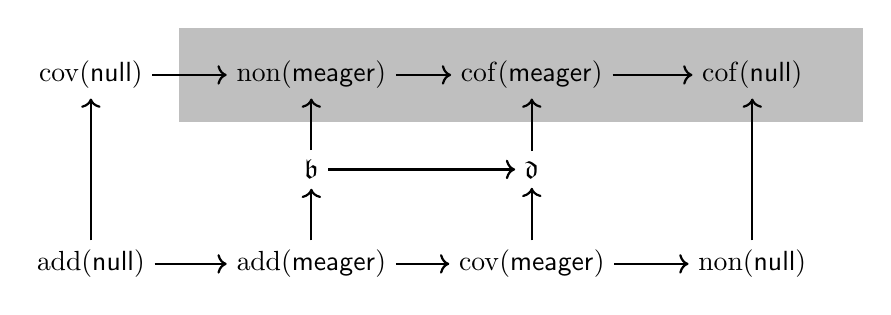
\begin{tikzpicture}
				\newcommand{\w}{2.8}
				\newcommand{\h}{1.2}
				\fill[very thick,gray!50!white] (\w*0.4, \h*2.5) rectangle (\w*3.5, \h*1.5);
				
				\node (addN) at (0, 0) {$\add(\nul)$};
				\node (covN) at (0, \h*2) {$\cov(\nul)$};
				
				\node (addM) at (\w, 0) {$\add(\meager)$};
				\node (b) at (\w, \h) {$\mathfrak{b}$};
				\node (nonM) at (\w, \h*2) {$\non(\meager)$};
				
				\node (covM) at (\w*2, 0) {$\cov(\meager)$};
				\node (d) at (\w*2, \h) {$\mathfrak{d}$};
				\node (cofM) at (\w*2, \h*2) {$\cof(\meager)$};
				
				\node (nonN) at (\w*3, 0) {$\non(\nul)$};
				\node (cofN) at (\w*3, \h*2) {$\cof(\nul)$};
				
				\draw[thick,->] (addN) to (covN);
				\draw[thick,->] (addN) to (addM);
				\draw[thick,->] (covN) to (nonM);	
				\draw[thick,->] (addM) to (b);
				\draw[thick,->] (b) to (nonM);
				\draw[thick,->] (addM) to (covM);
				\draw[thick,->] (nonM) to (cofM);
				\draw[thick,->] (covM) to (d);
				\draw[thick,->] (d) to (cofM);
				\draw[thick,->] (b) to (d);
				\draw[thick,->] (covM) to (nonN);
				\draw[thick,->] (cofM) to (cofN);
				\draw[thick,->] (nonN) to (cofN);
				
				
			\end{tikzpicture}
			\]
			
		この強制法は\cite{bjs}で考案され,その後テキスト\cite{bartoszynski1995set}にも載せられている.本稿はこの強制法のサーベイである.
	
	
	\section{強制法の性質}
	
	この節ははじめは読み飛ばして,必要に応じて戻ってくればよい.
	
	\subsection{Axiom Aとstrong axiom A}
	
	\begin{defi}
		強制概念$P$がaxiom Aを満たすとは$P$の順序の列$\seq{ \le_n : n \in \omega}$が存在して次の3条件を満たすことである.
		\begin{enumerate}[(1)]
			\item $q \le_{n+1} p$ならば$q \le_n p$かつ$q \le p$.
			\item $\seq{p_n : n \in \omega}$が$P$の元の列ですべての$n$で$p_{n+1} \le_n p_n$を満たすならば,$p \in P$が存在して,すべての$n$で$p \le_n p_n$である.
			\item $A \subset P$が反鎖ならば,すべての$p \in P$と$n \in \omega$に対して$q \le_n p$が存在して,$\{ r \in A : q \parallel r  \}$は可算.
		\end{enumerate}
		条件(3)の代わりに次の(3')を仮定したとき$P$はstrong axiom Aを満たすという.
		\begin{enumerate}[(3')]
			\item $A \subset P$が反鎖ならば,すべての$p \in P$と$n \in \omega$に対して$q \le_n p$が存在して,$\{ r \in A : q \parallel r  \}$は有限.
	\end{enumerate}

	\end{defi}

	\begin{fact}
		axiom Aを満たす強制概念はproperである.
	\end{fact}

	\begin{lem}
		strong axiom Aを満たす強制概念$P$は$\omega^\omega$-boundingである.すなわち
		\[
		P \forces (\forall f \in \omega^\omega)(\exists g \in \omega^\omega \cap V)(f \le g).
		\]
	\end{lem}
	\begin{proof}
		$p \in P$と名前$\dot{f}$で$p \forces \dot{f} \in \omega^\omega$なものをとる.
		各$n \in \omega$に対して,$A_n$を$\dot{f}(n)$の値を決定する条件からなる極大反鎖とする.
		条件の列$\seq{p_n : n \in \omega}$を次を満たすように取る.
		\begin{itemize}
			\item $p_0 \le p$.
			\item $p_{n+1} \le_n p_n$.
			\item $\{ r \in A_n : p_n \parallel r \}$は有限.
		\end{itemize}
		これは(3')より取れる.最後に$q$を$\seq{p_n : n \in \omega}$のfusionとする.
		
		今,有限集合$\{ r \in A_n : p_n \parallel r \}$に対応する$\dot{f}(n)$の値の候補の全体を$B_n$とする:
		\[
		B_n = \{ m \in \omega : (\exists r \in A_n) (p_n \parallel r \land r \forces \dot{f}(n) = m) \}.
		\]
		$B_n$は有限集合なので$g(n) = \max B_n$とおく.
		このとき$q \forces (\forall n \in \omega)(\dot{f}(n) \le g(n))$である.
		
		実際,$n \in \omega$とする.
		$q' \le q$を任意にとる.
		$A_n$が極大反鎖なので$r \in A_n$があって,$q' \parallel r$.
		$q'$は$p_n$より下にあるので,$r$は$p_n$とも両立する.
		よって,$r \forces \dot{f}(n) \in B_n$.特に$r \forces \dot{f}(n) \le g(n)$である.
		$q'$と$r$の共通拡大$s$をとると,$s \forces \dot{f}(n) \le g(n)$でもあるので,これで$q \forces (\forall n \in \omega)(\dot{f}(n) \le g(n))$が示された.
	\end{proof}

	\begin{lem}
		\begin{enumerate}
		\item $P$を強制概念とする.axiom Aの条件(3)は次と同値である.
		\[
		(\forall \dot{a} \in V^P)(\forall p \in P)(\forall n \in \omega)(p \forces \dot{a} \in V \Rightarrow (\exists x \text{可算集合})(\exists q \le_n p)(q \forces \dot{a} \in x))
		\]
		\item $P$を強制概念とする.strong axiom Aの条件(3')は次と同値である.
		\[
		(\forall \dot{a} \in V^P)(\forall p \in P)(\forall n \in \omega)(p \forces \dot{a} \in V \Rightarrow (\exists x \text{有限集合})(\exists q \le_n p)(q \forces \dot{a} \in x))
		\]
		\end{enumerate}
	\end{lem}

	\subsection{性質$\mathrm{B}_{f, h}$と$(f, h)$-bounding}
	
	\begin{defi}
		強制概念$P$はaxiom Aを満たすとする.$f \in \omega, h \in \omega^{\omega \times \omega}$とする.各$n \in \omega$について
		\[
		\lim_{k \to \infty} \frac{h(k, n)^n}{f(k)} = 0
		\]
		と仮定する.$P$が性質$\mathrm{B}_{f, h}$を持つとは,
		\begin{align*}
			&(\forall p \in P)(\forall n \in \omega)(\exists c, l \in \omega)(\forall m \ge l)(\forall r \in \omega)(\forall \dot{B} \in V^P) \\
			& \hspace{0.5cm} (T \forces (\dot{B} \subset f(m) \AND \abs{\dot{B}} \le r) \rightarrow \\
			& \hspace{1cm} (\exists q \le_n p)(\exists A \subset f(m))(\abs{A} \le c \cdot h(m, n) \cdot r \AND q \forces \dot{B} \subset A)).
		\end{align*}
		を満たすこととする.
	\end{defi}
	
	
	\begin{defi}
		$f, h \in \omega^\omega$は
		\[
		\lim_{n \to \infty} \frac{h(n)^n}{f(n)} = 0
		\]
		を満たすとする.強制概念$P$が$(f, h)$-boundingであるとは,
		\[
		P \forces (\forall x \in \prod_n f(n))(\exists S \in V \cap ([\omega]^{<\omega})^\omega)(\forall n)(\abs{S(n)} \le h(n) \AND f(n) \in S(n))
		\]
		を満たすことである.
	\end{defi}
	
	\begin{lem}
		$\mathrm{B}_{f, h}$を満たす強制概念は$(f, h^*)$-boundingである.ここに
		\[ h^*(n) = h(n, n). \]
	\end{lem}
	\begin{proof}
		$p \in P$, $\dot{x} \in V^P$で$p \forces \dot{x} \in \prod_n f(n)$とする. \todo
	\end{proof}
	
	\begin{fact}
		各iterandが「properかつ$(f, h)$-bounding」な強制法の加算台反復はproperかつ$(f, h)$-boundingである.
	\end{fact}

	\begin{lem}
	$(f, h)$-boundingな強制法はランダム実数を付け加えない.
	\end{lem}
	\begin{proof}
		$\{ I_n : n \in \omega\}$を$\omega$の区間分割で$\abs{I_n} = f(n)$なものとする.
		$p \forces \dot{y} \in 2^\omega$とする.
		$p \forces \dot{x}(n) = \dot{y} \upharpoonright I_n$なる名前$\dot{x}$を定める.
		すると$(f, h)$-boundingより$q \le p$と$S$がとれて,各$n \in \omega$について
		\[
		\abs{S(n)} \le h(n) \AND q \forces \dot{x}(n) \in S(n).
		\]
		今,
		\[
		q \forces \dot{A} = \{ z \in 2^\omega : (\forall n)(z \upharpoonright I_n \in S(n)) \}	
		\]
		とおくと,$q \forces \dot{y} \in \dot{A}$であり,また
		\begin{align*}
		\mu(\dot{A}) &\le \mu(\{ z \in 2^\omega : z \upharpoonright I_n \in S(n) \}) \\
		&\le \frac{h(n)}{2^{f(n)}} \\
		&\le \frac{h(n)^n}{f(n)} \to 0\ (n \to \infty) 
		\end{align*}
		であるので,$\dot{A}$は測度$0$である.また,$\dot{A}$は$V$の元でコードできる閉集合である.
		よって,$\dot{y}$はランダム実数ではない.
	\end{proof}
	
	\subsection{$\sqsubseteq^{\mathrm{random}}$について}
	
	\section{$\PTfg$について}
		
	\begin{asm}\label{fgassumption}
		この節では$f \in \omega^\omega$と$g \in \omega^{\omega \times \omega}$は次の条件を満たす関数とする.
		\begin{enumerate}
			\item すべての$n \in \omega$に対して$f(n) > \prod_{j < n} f(j)$.
			\item すべての$n, j \in \omega$に対して$g(n, j+1) > f(n) \cdot g(n, j)$.
			\item $\min \{ j \in \omega : g(n, j) > f(n+1) \} \to \infty$ (as $n \to \infty$)
		\end{enumerate}
	\end{asm}

	このような関数$f, g$は存在する.
	(3)を満たすためには$\min \{ j \in \omega : g(n, j) > f(n+1) \} \ge n+1$であれば十分なことに注意する.
	つまり,$g(n, 0), g(n, 1), \dots, g(n, n) < f(n+1) < g(n, n+1)$であればよい.
	そこで番号の小さい方から値を順に定めていくことができる.
	
	詳しくは次の図のような順番で定めていけばよい.
	\begin{figure}[h]\label{fig:ordering}
		\caption{$f$と$g$を定める順番}
	\[
	\tikz{
		\draw[->] (1, 0) -- (5, 0) node[right] {$j$};
		\draw[->] (1, 0) -- (1, 5) node[above] {$n$};
		\draw[->] (0, 0) -- (0, 5) node[above] {$n$};
		\node at (-1, 5) {$f(n)$};
		\node at (5, 5) {$g(n, j)$};
		
		\fill (0,0.5) circle (0.1) node[left] {$0$};
		\fill (1.5,0.5) circle (0.1) node[left] {$1$};
		\fill (0,1.5) circle (0.1) node[left] {$2$};
		\fill (1.5,1.5) circle (0.1) node[left] {$3$};
		\fill (2.5,0.5) circle (0.1) node[left] {$4$};
		\fill (2.5,1.5) circle (0.1) node[left] {$5$};
		\fill (0,2.5) circle (0.1) node[left] {$6$};
		\fill (1.5,2.5) circle (0.1) node[left] {$7$};
		\fill (2.5,2.5) circle (0.1) node[left] {$8$};
		\fill (3.5,0.5) circle (0.1) node[left] {$9$};
		\fill (3.5,1.5) circle (0.1) node[left] {$10$};
		\fill (3.5,2.5) circle (0.1) node[left] {$11$};
		
		\draw (0,0.5) -- (1.5,0.5) -- (0, 1.5) -- (1.5,1.5) -- (2.5,0.5) -- (2.5,1.5) -- (0,2.5) -- (1.5,2.5) -- (2.5,2.5) -- (3.5, 0.5) -- (3.5, 1.5) -- (3.5, 2.5);
		
		\node at (-0.1, 3.3) {$\vdots$};
		\node at (2, 3.3) {$\vdots$};
		\node at (4.5, 3.3) {$\reflectbox{$\ddots$}$};
		\node at (4.5, 1.5) {$\cdots$};
	}
	\]
	\end{figure}

	
	\begin{defi}
		木$T \subset \omega^{<\omega}$に対して$\stem(T)$をその幹,すなわちその上で分岐する最初のノードとする.
		木$T \subset \omega^{<\omega}$とそのノード$s \in T$に対して
		\[
		T_s = \{ t \in T : s \le t \OR t \le s \}
		\]
		とおく.
	\end{defi}
		
	\begin{defi}
		集合$\Seq^f$を$\Seq^f  = \{ s \in \omega^{<\omega} : (\forall j < \abs{s}) (s(j) \le f(j)) \}$と定める.
		$\PTfg$を次で定められる強制概念とする.
		$T \in \PTfg$であるのは次のとき:
		\begin{enumerate}
			\item $T$は$\Seq^f$の完全な部分木.
			\item 関数$r \in \omega^\omega$で$\lim_{n \to \infty} r(n) = \infty$なものが存在して,次を満たす:
			\[
			(\forall s \in T)(\stem(T) \subset s \rightarrow \abs{\suc_T(s)} \ge g(\abs{s}, r(\abs{s}))).
			\]
		\end{enumerate}
		
		$\PTfg$の元の順序は包含で定められる:$S, T \in \PTfg$について$T \le S \Leftrightarrow T \subset S$.
	\end{defi}

	\subsection{$\PTfg$は$\non(\meager)$を上げる}

	\begin{lem}
		$\PTfg \forces V \cap \omega^\omega \in \meager$.
	\end{lem}
	\begin{proof}
		$G$を$(V, \PTfg)$ジェネリックフィルターとする.
		$f_G = \bigcup \{ \stem(T) : T \in G \}$とする.
		すると
		\[
		(\forall h \in V \cap \omega^\omega)(\forall^\infty n)(h(n) \ne f_G(n))
		\]
		である.
		実際,$h \in V \cap \omega^\omega$に対して
		\[
		D_h = \{ T \in \PTfg : (\forall s \in T)(\stem(T) \subset s \rightarrow s(\abs{s}-1) \ne h(\abs{s}-1)) \}
		\]
		とおくとこれは$V$内で定められる稠密集合である.稠密性を今から確かめよう.
		
		$T \in \PTfg$とする.
		すると$r \in \omega^\omega$で$\lim_{n \to \infty} r(n) = \infty$であって
		\[
		(\forall s \in T)(\stem(T) \subset s \rightarrow \abs{\suc_T(s)} \ge g(\abs{s}, r(\abs{s})))
		\]
		を満たす.
		$r'(n) = r(n) - 1$とおくと仮定\ref{fgassumption} (2)より,ある$n_0$があって,すべての$n \ge n_0$で
		\[
		g(n, r(n)) - 1 \ge g(n , r'(n))
		\]
		が言える.
		$T' \subset T$をまず幹の高さを$n_0$以上にして,次に幹の高さ以上の$h$と同じ値のラベルを取るノードを削った木とする.
		今,
		\[
		\suc_{T'}(s) \ge \suc_T(s) - 1 \ge g(\abs{s}, r(\abs{s})) - 1 \ge g(\abs{s}, r'(\abs{s}))
		\]
		であるので,$r'$は$T'$が$\PTfg$の元であることを目撃する.
		これで,$D_h$の稠密性が言えた.
		
		以上より
		\[
		V \cap \omega^\omega \subset \{ h \in \omega^\omega : (\forall^\infty n)(h(n) \ne f_G(n)) \} \in \meager
		\]
		である.
		\end{proof}

	\subsection{$\PTfg$はproperかつ$\omega^\omega$-bounding}

	$T \in \PTfg$について,$r_T$で$r$であって条件(2)を目撃し,$r(i) = 0$ for all $i < \abs{\stem{T}}$を満たすものの中で最大なものを表す.
	
	\begin{defi}
		\begin{align*}
		\PTfg^* = \{ T \in \PTfg : r_T \text{ is non-decreasing} \AND (\forall s \in T)(\stem(T) \subset s \rightarrow \abs{\suc_T(s)} = g(\abs{s}, r_T(\abs{s}))) \}.
		\end{align*}
	\end{defi}

	\begin{lem}
		$\PTfg^*$は$\PTfg$の稠密部分集合である.
	\end{lem}
	\begin{proof}
			$T \in \PTfg$をとる.
			$\lim r_T = \infty$より,各$k \in \omega$について$i_k \in \omega$があって$(\forall i \ge i_k) (r_T(i) \ge k)$.
			$(i_k : k \in \omega)$は単調増大としてよい.
			$r' \in \omega^\omega$を
			\[
			r'(i) = k \ \ (i \in [i_k, i_{k+1}))
			\]
			とおくと$r'$は非減少かつ$\infty$に発散し,$r' \le r'$である.
			$T$の中のノードをいくつか消して$\suc_{T'}(s) = g(\abs{s}, r'(\abs{s}))$なる部分木$T'$を作る.
			すると$T' \le T$,$r_{T'} = r'$かつ$T' \in \PTfg^*$である.
	\end{proof}
	
	\begin{defi}
		$S, T \in \PTfg^*$と$n \in \omega$に対して関係$T \le_n S$を次で定める:
		\begin{align*}
			T \le_n S \Leftrightarrow T \le S \AND (\forall i \in \omega) (T \cap \omega^{i+1} \ne S \cap \omega^{i+1} \rightarrow r_{T'}(i) \ge n).
		\end{align*}
	\end{defi}
	
	\begin{lem}
		$\seq{T^n : n \in \omega}$を$\PTfg^*$の元の列であって,$T^{n+1} \le_{n} T^n$ for $n \in \omega$なものとする.
		すると$T \in \PTfg^*$があって,$T \le_{n} T^n$ for all nを満たす.
	\end{lem}
	\begin{proof}
		$n \in \omega$に対して,$u_n = \min \{ j \in \omega : r_{T^{n+1}}(j) \ge n \}$とおく.
		木$T$を
		\[
		T = \bigcup_{n \in \omega} (T^n \cap \omega^{\le u_n}).
		\]
		により定める.
		
		\begin{claim}{A}
			各$u_n$はwell-definedである.
		\end{claim}
		\begin{claimproof}
			これは$r_{T^n}(j) \to \infty\ (j \to \infty)$から従う.
		\end{claimproof}
	
		\begin{claim}{B}
		$u_n \le u_{n+1}$.
		\end{claim}
		\begin{claimproof}
			$r_{T^{n+1}} \le r_{T^n}$より,もし$r_{T^{n+1}}(j) \ge n$ならば$r_{T^n}(j) \ge n$である.
		\end{claimproof}
	
		\begin{claim}{C}
			$\lim_{n \to \infty} u_n = \infty$.
		\end{claim}
		\begin{claimproof}
			$k \in \omega$を固定する.
			すると$n_0 \in \omega$を取れて$f(k) < g(k, n_0)$を満たす.
			このとき各$n > n_0$について
			\begin{align*}
				g(k, r_{T^n}(k)) \le f(k) \le g(k, n_0)
			\end{align*}
			を得る,なぜなら我々の木は$\Seq^f$の部分木だからである.
			よって,$g$の単調性より,$r_{T^n}(k) \le n_0 < n$を得る.
			ゆえに$u_n > k$.
		\end{claimproof}
		
		\begin{claim}{D}
			各$n \in \omega$について,$T^n \cap \omega^{\le u_n} = T^{n+1} \cap \omega^{\le u_n}$.
		\end{claim}
		\begin{claimproof}
			$s \in T^n \cap \omega^{\le u_n}$を取る.
			$t$を$s$の前者とする.
			$s \not \in T^{n+1}$だとする.
			すると,$T^n \cap \omega^{\abs{t}+1} \ne T^{n+1} \cap \omega^{\abs{t}+1}$.
			よって,$T^{n+1} \le_n T^n$より,$r_{T^{n+1}}(\abs{t}) \ge n$を得る.
			したがって,$u_n \le \abs{t}$.
			これは$\abs{t} < \abs{s} \le u_n$に矛盾する.
		\end{claimproof}
	
		\begin{claim}{E}
			$T \in \PTfg^*$.	
		\end{claim}
		\begin{claimproof}
			主張Dより
			\[
			r_{T^{m+1}}(k) = r_{T^{n+1}}(k) \text{ (if $k \le u_{m+1}, u_{n+1}$)}.
			\]
			である.
			よって,$r \in \omega^\omega$を式
			\[
			r(k) = r_{T^{n+1}}(k) \text{ (if $k \le u_{n+1}$)}.
			\]
			によって定められる.
			この$r$は非減少であり,$\lim_{n \to \infty} r(n) = \infty$を満たす.
			$s \in T$を取る.
			すると$n \in \omega$であって,$s \in T^{n+1} \cap \omega^{\le u_{n+1}}$を満たすものを取れる.
			このとき,
			\[
			\abs{\suc_T(s)} = \abs{\suc_{T^{n+1}}(s)} = g(\abs{s}, r_{T^{n+1}}(\abs{s})) = g(\abs{s}, r(\abs{s})).
			\]
			よって,$T \in \PTfg^*$.
		\end{claimproof}
	
		\begin{claim}{F}
			すべての$n$について,$T \le_n T^n$.
		\end{claim}
		\begin{claimproof}
			$n \in \omega$を固定する.
			$t \in T$とする.
			すると$m \in \omega$が取れて,$t \in T^m \cap \omega^{\le u_m}$を満たす.
			もし$m \ge n$ならば,$t \in T^m \subset T^n$である.
			もし$m < n$ならば,$t \in T^m \cap \omega^{\le u_m} \subset T_n \cap \omega^{\le u_n} \subset T_n$である.
			よって$T \subset T^n$を得る.
			
			また,$T \cap \omega^{\le u_n} = T^n \cap \omega^{\le u_n}$である.
			
			$i \in \omega$を固定し,$T \cap \omega^{i+1} \ne T^n \cap \omega^{i+1}$を仮定する.
			すると$i \ge u_n$である.
			自然数$m$を$i < u_{m+1}$を満たす最小としてとる.
			よって,$u_m \le i < u_{m+1}$.
			すると$u_n \le i < u_{m+1}$より$n \le m$を得る.
			
			ゆえに$u_m$の定義より,$r_{T^{m+1}}(i) \ge m \ge n$を得る.
			したがって,$r_T(i) \ge n$.
		\end{claimproof}
	
		これで補題の証明が終わった.
		\end{proof}
	
	\begin{lem}\label{shrinkinglemma}
		任意の$r \in \omega^\omega$で$\lim r = \infty$なものと$n \in \omega$に対して,$r' \in \omega^\omega$で$\lim r' = \infty$なものが存在して有限個を除いたすべての$k \in \omega$で
		\[
		g(k, r(k)) - g(k, n) \ge g(k, r'(k)).
		\]
	\end{lem}
	\begin{proof}
		$r'(k) = r(k) - n$が条件を満たす.実際,仮定\ref{fgassumption} (2)より,十分大きな$k$について
		\begin{align*}
			g(k, r(k)) &> f(k) \cdot g(k, r(k) - 1) \\
			&> f(k)^2 \cdot g(k, r(k) - 2) \\
			&> \dots \\
			&> f(k)^n \cdot g(k, r(k) - n) \\
			&> 2 \cdot g(k, r(k) - n) \\
			&> g(k, r(k) - n) + g(k, n)
		\end{align*}
	が成り立つ.
	\end{proof}
		
	\begin{lem}\label{ptfg-strong-axiom-a}
		$T \in \PTfg^*$かつ$n \in \omega$とする.
		$T \forces \dot{a} \in V$とする.
		すると$\tilde{T} \le_n T$と$m \in \omega$があって,
		\[
		(\forall s \in \tilde{T} \cap \omega^m) (\exists a) (\tilde{T}_s \forces \dot{a} = a).
		\]
	\end{lem}
	\begin{proof}
		集合$S$を次で定める:
		\[
		S = \{ t \in T : (\exists m \in \omega)(\exists \tilde{T} \le_n T_t)(\forall s \in \tilde{T} \cap \omega^m)(\tilde{T}_s \text{ decides } \dot{a}) \}.
		\]
		\begin{claim}{A}
			$t \in T$とする.$t \not \in S$ならば$\abs{\suc_T(t) \cap S} < g(\abs{t}, n)$.
		\end{claim}
		\begin{claimproof}
			対偶を示す.
			$\abs{\suc_T(t) \cap S} \ge g(\abs{t}, n)$と仮定する.
			$\suc_T(t) \cap S = \{s_1, \dots, s_l\}$としよう.
			各$s_i$は$S$の元だから,$m_i \in \omega$と$\tilde{T}^i \le_n T_{s_i}$がとれて,
			\[
			(\forall s \in \tilde{T}^i \cap \omega^m)((\tilde{T}^i)_s \text{ decides } \dot{a})
			\]
			となる.$m$を$m = \max \{ m_1, \dots, m_l \}$で定め,
			\[
			\tilde{T} = \bigcup_{1 \le i \le l} \tilde{T}^i.
			\]
			とおく.
			$\tilde{T}$を縮めると$\tilde{T} \in \PTfg^*$かつ$\tilde{T} \le_n T_s$かつ$(\forall s \in \tilde{T} \cap \omega^m)(\tilde{T}_s \text{ decides } \dot{a})$を得る.
			
			よって$t \in S$を得る.
		\end{claimproof}
	
		\begin{claim}{B}
			$t \in T$とする.
			このとき$t \not \in S$ならば$(\exists s \in \suc_T(t)) (s \not \in S)$.
		\end{claim}
		\begin{claimproof}
			主張Aと似た議論で示せる.
		\end{claimproof}
	
		補題を示すために,背理法により$\stem(T) \not \in S$を仮定する.
		木$\tilde{S} \le T$をレベルに関する帰納法で
		\[
		\suc_{\tilde{S}}(s) = \suc_T(s) \setminus S \text{ ($s \in \tilde{S}$)}
		\]
		と定める.
		
		主張Bより$s \in \tilde{S}$に対して$\suc_{\tilde{S}}(s) = \emptyset$は起こり得ない.
		そして主張Aより$\tilde{S}$の中で各高さ$k$と高さ$k$の各ノードに対して切り落とされた後続者の数は$g(k, n)$で抑えられる.よって補題\ref{shrinkinglemma}より$\tilde{S} \in \PTfg$である.
		
		$\tilde{S}_1 \le \tilde{S}$と$a$であって$\tilde{S}_1 \forces \dot{a} = a$なものを取る.
		
		$t \in T$と$\tilde{S}_2 \le \tilde{S}_1$であって$\tilde{S}_2 \le_n T_t$かつ$t \in \tilde{S}_2$なものを取る.
		すると$m =\abs{t}$と$\tilde{S}_2$は$t \in S$を目撃する.
		しかし$t \in \tilde{S}_2 \subset \tilde{S}$であるので,よって$t \not \in S$である.これは矛盾.
	\end{proof}
	
	\begin{cor}
		$\PTfg$はstrong axiom Aを満たす.
	\end{cor}

	\subsection{$\PTfg$は$\cov(\nul)$を保つ}
	
	次の定理は$\PTfg$の反復がランダム実数を付け加えないこと ($\cov(\nul)$を保つこと)を保証するものである.
	
	\begin{thm}
		$f \in \omega^\omega, g, h \in \omega^{\omega\times\omega}$は仮定\ref{fgassumption}に加えて次の条件も満たすとする.
		\begin{enumerate}[(A)]
			\item すべての$n, j \in \omega$について$g(n, j+1) > f(n)^{f(n)} \cdot g(n, j)$.
			\item すべての$n, k \in \omega$について$h(n, k) \ge \prod_{i < n} g(i, k)$.
			\item すべての$r, c, k \in \omega$について$(\forall^\infty n)(c \cdot h(n, k)^r \le f(n)/2)$.
		\end{enumerate}
		このとき$\PTfg$は性質$\mathrm{B}_{f, h}$を満たす.
		すなわち,
		\begin{align*}
		&(\forall T \in \PTfg)(\forall n \in \omega)(\exists c, l \in \omega)(\forall m \ge l)(\forall r \in \omega)(\forall \dot{B} \in V^{\PTfg}) \\
		& \hspace{0.5cm} (T \forces (\dot{B} \subset f(m) \AND \abs{\dot{B}} \le r) \rightarrow \\
		& \hspace{1cm} (\exists T' \le_n T)(\exists A \subset f(m))(\abs{A} \le c \cdot h(m, n) \cdot r \AND T' \forces \dot{B} \subset A)).
		\end{align*}
	\end{thm}

	仮定\ref{fgassumption}の(1)-(3)と(A)-(C)を満たす関数$f, g, h$が存在することを見よう.
	$f, g$の定義の順番は図\ref{fig:ordering}の順番の通りにする.
	$g(n, k)$が定義された時点で,$h(n + 1, k)$を$h(n + 1, k) = \prod_{i \le n} g(i, k)$と定める.
	このように$h$を定めて,かつ条件(C)の「十分大なすべての$n$について」という部分を「すべての$n \ge r + c + k + 1$について」と強めると条件(C)は
	\[
	f(n) \ge 2 n \cdot h(n, n-1)^n
	\]
	で十分である.ところが$h$の定め方より
	\[
	f(n) \ge 2 n \cdot \prod_{i < n} g(i, n-1)^n
	\]
	となれば良い.この右辺に登場する$g$の値は全て$f(n)$を定義する前に決めているので,$f(n)$を決める段階でこの不等式も要請すればよい.
	
	\begin{proof}
		$T \in \PTfg$, $n \in \omega$とする.
		$l \in \omega$を
		\[
		(\forall s \in T)(|s| > l \rightarrow \abs{\suc_T(s)} > g(\abs{S}, n+1))
		\]
		なるようにとる.
		$c = \abs{T \cap \omega^l}$ととる.
		$m \ge l$と$r \in \omega$が与えられたとして
		\[
		T \forces \dot{B} = \{\dot{b}_1, \dots, \dot{b}_r\} \subset f(m)
		\]
		とする.
		
		補題\ref{ptfg-strong-axiom-a}より,$k \in \omega$と$\tilde{T} \le_{n+1} T$が取れて,
		\[
		(\forall j \le  r)(\forall s \in \tilde{T} \cap \omega^k)(\exists a^j_s \in \omega)(\tilde{T}_s \forces \dot{b}_j = a^j_s) \tag{$\ast$}
		\]
		となる.$k$は大きく取り直せるので,$k \ge m$としてよい.
		
		列$\tilde{T} = T^k \ge_n T^{k-1} \ge_n \dots \ge_n T^m$を次のように構成する.
		$T^{z+1}$が構成されたとする.$T^z$を$T^{z+1}$の長さ$z$の列を後続者をいくつか取り除くことで得る.
		$z$に関する帰納法の仮定を次とする.
		\[
		(\forall t \in T^{z+1} \cap \omega^{z+1})(\exists B^t \subset f(m))(\abs{B^t} = r \AND T^{z+1}_t \forces \dot{B} = B^t).
		\]
		$z+1 = k$では($\ast$)より良い.
		
		$s \in T^{z+1} \cap \omega^z$とする.
		$B$を$\{ B^t : t \in \suc_{T^{z+1}}(s)\}$の中でもっとも多く現れる集合とする.
		\[
		\suc_{T^z}(s) = \{ t \in \suc_{T^{z+1}} : B^t = B \}
		\]
		とおく.
		
		今,$s \in T^z \cap \omega^z$ならば
		\[
		\abs{\suc_{T^z}(s)} \ge \frac{g(z, n+1)}{f(m)^r}
		\]
		である.右辺の分母は$B$の選び方の個数,分子は$\suc_{T^z}(s)$の個数である.一番頻出する$B$を選んでいたおかげでこの不等号が成立する.
		したがって,	
		\[
		\abs{\suc_{T^z}(s)} \ge \frac{g(z, n+1)}{f(m)^r} \ge \frac{g(z, n+1)}{f(z)^f(z)} \ge g(z, n)
		\]
		を得る.最後の不等式は仮定(A)によるものである.
		よって,$T^z \ge_n T^{z+1}$を得る.
		
		最後に$\tilde{\tilde{T}} = T^m$とおく.
		$T^m$の構成の仕方より
		\[
		(\forall j \le r)(\exists s \in \tilde{\tilde{T}} \cap \omega^m)(\exists a^j_s \in f(m))(\tilde{\tilde{T}}_s \forces \dot{b}_j = a^j_s)
		\]
		を得る.また,
		\[
		\abs{\tilde{\tilde{T}} \cap \omega^m} \le c \cdot g(l+1, n) \cdot \dots \cdot g(m, n) \le c \cdot h(m, n)
		\]
		を得る.一つ目の不等号は$c = \abs{T \cap \omega^l}$だから各高さで分岐する数を掛けていけば高さ$m$のノードの数が抑えられるからである.二つ目は仮定(B)による.
		
		最後に
		\[ A = \{a^j_s  : s \in \tilde{\tilde{T}} \cap \omega^m \AND j \le r \} \]
		とおけば,
		\begin{align*}
		\abs{A} &\le c \cdot h(m, n) \cdot r \\
		\tilde{\tilde{T}} &\le_n T \\
		\tilde{\tilde{T}} &\forces \dot{B} \subset A
		\end{align*}
		を得る.
	\end{proof}

	\subsection{$\PTfg$は$\non(\nul)$を保つ}
	
	\begin{thm}
		$A \subset 2^\omega$は$\mu^*(A) > 0$ (外測度正)を満たすとする.
		すると$\PTfg \forces \mu^*(A) > 0$.
	\end{thm}
	\begin{proof}
		$c = \mu^*(A) > 0$とおく.
		背理法で結論の否定を仮定する.
		すると$T \in \PTfg$と有理区間の名前の列$\seq{\dot{I}_n : n \in \omega}$があって,次を満たす:
		\begin{enumerate}
			\item $T \forces \sum_{n=1}^\infty \mu(\dot{I}_n) < \infty$.
			\item $T \forces A \subset \bigcap_{m \in \omega} \bigcup_{n > m} \dot{I}_n$.
		\end{enumerate}
		$s_0 = \stem(T)$とおく.補題\ref{ptfg-strong-axiom-a}より次のような自然数の単調増加列$\seq{k_n : n \in \omega}$が取れると仮定して良い.
		\begin{enumerate}
			\item 各$s \in T \cap \omega^{k_n}$について,$T_s$は$\dot{I}_j$ (for $j \le n$)の値を決めている.
			\item $T \forces \sum_{n \ge \abs{s_0}} \mu(\dot{I}_n) < c/2$.
		\end{enumerate}
	
		各$s \in T \cap \omega^{k_n}$と$j \le n$について
		\[
		I^s_j = \begin{cases}
			I & \text{if $T_s \forces \dot{I}_j = I$} \\
			\emptyset & \text{otherwise}
		\end{cases}
		\]
		と定める.
		
		$r \in \omega^\omega$が$T \in \PTfg$を目撃するとする.
		$r' \in \omega^\omega$で$r'(n) \le r(n)$かつ$r'(n) \to \infty$なものを考える.
		
		\begin{lem}\label{finitetree}
			$x \in 2^\omega$について次は同値.
			\begin{enumerate}
				\item $\tilde{T} \le T$があって$r'$は$\tilde{T} \in \PTfg$を目撃し,かつ$\tilde{T} \forces x \not \in \bigcup_{n \in \omega} \dot{I}_n$.
				\item どんな$k \ge \abs{s_0}$についても,有限の木$\mathbf{t}$が存在して,次を満たす:
				\begin{enumerate}
					\item $\mathbf{t} \subset T \cap \omega^{\le k}$.
					\item すべての$s \in \mathbf{t} \cap \omega^{\ge\abs{s_0}}$について$\abs{\suc_\mathbf{t}(s)} \ge g(\abs{s}, r'(\abs{s}))$
					\item もし$s \in \mathbf{t} \cap \omega^k$ならば$x \not \in \bigcup_{j \in \omega} I^s_j$.
				\end{enumerate}
			\end{enumerate}
		\end{lem}
		\begin{proof}
			(1) $\rightarrow$ (2)について.もし$\tilde{T}$が(1)を満たすならば,$\mathbf{t} = \tilde{T} \upharpoonright k$は(2)を満たす.
			(2) $\rightarrow$ (1)について.コンパクト性定理を使えば(1)の$\tilde{T}$の存在が言える.
		\end{proof}
	
		今集合$D \subset 2^\omega$を次で定める:$y \in D$であるのは$\tilde{T} \in \PTfg$が存在して次を満たすとき
		\begin{enumerate}
			\item $\tilde{T} \le T$かつ$\stem(\tilde{T}) = s_0$
			\item $\tilde{T} \forces y \not \in \bigcup_{n \ge \abs{s_0}} \dot{I}_n$
			\item $(\forall n \ge \abs{s_0})(\forall s \in \tilde{T} \cap \omega^n)(\abs{\suc_{\tilde{T}}(s)} \ge g(n, r(n)-1))$.
		\end{enumerate}
		また各$k \ge \abs{s_0}$について集合$D_k \subset 2^\omega$を次で定める:$y \in D_k$であるのは有限な木$\mathbf{t}$が存在して次を満たすとき
		\begin{enumerate}
			\item $\mathbf{t} \subset T \cap \omega^{\le k}$.
			\item $(\forall n \ge \abs{s_0})(\forall s \in \mathbf{t} \cap \omega^n)(\abs{\suc_{\mathbf{t}}(s)} \ge g(n, r(n)-1))$.
			\item $(\forall s \in \mathbf{t} \cap \omega^k)(y \not \in \bigcup_{n \ge \abs{s_0}} I^s_n)$.
		\end{enumerate}
	
		上の補題\ref{finitetree}より$D = \bigcap_{k \in \omega} D_k$である.
		$D_k$は定義より明らかにBorel集合であるため,$D$もBorel集合,特にLebesgue可測である.
		
		また,$D$の定義より$D \cap A = \emptyset$である.
		よって,
		\[c = \mu^*(A) \leq \mu(2^\omega \setminus D)\]
		となる.
		
		$D_k$は減少列であるため,測度の連続性より$k \in \omega$があって,
		\[
		\mu(2^\omega \setminus D_k) > 3c / 4
		\]
		を得る.
		
		次に各$k \in \omega$と各$s \in T$であって,$\abs{s_0} \le \abs{s} \le k$なものについて,集合$D_{k,s}$を次で定める:$y \in D_{k,s}$であるのは有限な木$\mathbf{t}$が存在して次を満たすとき
		\begin{enumerate}
			\item $\mathbf{t} \subset T \cap \omega^{\le k}$.
			\item $(\forall n \ge \abs{s})(\forall v \in \mathbf{t} \cap \omega^n)(\abs{\suc_{\mathbf{t}}(v)} \ge g(n, r(n)-1))$.
			\item $(\forall v \in \mathbf{t} \cap \omega^k)(y \not \in \bigcup_{n \ge \abs{s_0}} I^s_n)$.
		\end{enumerate}
	定義より$D_k = D_{k, s_0}$は明らか.また,$D_{k, s}$と$\bigcup_{n \ge \abs{s_0}} I^s_n$は交わらないので,
	\[
	\mu(2^\omega \setminus D_{k, s}) \le \sum_{n \ge \abs{s_0}} \mu(I^s_n) < \frac{c}2
	\]
	である.
	
	\begin{lem}
		$a$を非負実数とする.
		$\abs{s_0} \le m < k$とし,$s \in T \cap \omega^m$と仮定する.
		各$t \in \suc_T(s)$について$\mu(2^\omega \setminus D_{k, t}) \le a$と仮定する.
		このとき
		\[
		\mu(2^\omega \setminus D_{k,s}) \le a \cdot \left(1-\frac1{f(m)} \right).
		\]
	\end{lem}
	\begin{proof}
		はじめに,$t \in \suc_T(s)$であって$y \in D_{k,t}$であるものの個数が$g(m, r(m) - 1)$以上であれば,それらを目撃する有限木を貼り合わせることにより,$y \in D_{k, s}$が分かる.
		対偶をとれば,
		\[
		y \not \in D_{k,s} \Rightarrow \abs{\{t \in \suc_T(s) : y \not \in D_{k,t}\}} \ge g(m, r(m)) - g(m, r(m)-1)
		\]
		となる.この逆
		\[
		y \in D_{k,s} \Rightarrow \abs{\{t \in \suc_T(s) : y \not \in D_{k,t}\}} < g(m, r(m)) - g(m, r(m)-1)
		\]
		も分かるので,
		\[
		y \not \in D_{k,s} \Leftrightarrow \abs{\{t \in \suc_T(s) : y \not \in D_{k,t}\}} \ge g(m, r(m)) - g(m, r(m)-1) \tag{$\ast$}
		\]
		を得る.
		
		次の簡単な補題を使う:
		\begin{lem}
			$N_1 > N_2$を二つの自然数とし,$\{A_j : j \le N_1\}$を測度$\le a$の集合の族とする.
			$A = \{ x \in 2^\omega : \text{$x$は$A_j$の中の少なくとも$N_2$個に入る} \}$とおく.
			すると$\mu(A) \le a \cdot \frac{N_1}{N_2}$.
		\end{lem}
		\begin{proof}
			$\chi_{A_i}$を$A_i$の特性関数とする.
			今,
			\[
			\int \sum_{i \le N_1} \chi_{A_i} \le N_1 \cdot a
			\]
			なので,
			\[
			\mu(\{ x \in 2^\omega : \sum_{i \le N_1} \chi_{A_i}(x) \ge N_2 \}) \le \frac{N_1 \cdot a}{N_2}.	
			\]
		\end{proof}
	
		この補題と($\ast$)を使えば,
		\[
		\mu(2^\omega \setminus D_{k,s}) \le a \cdot \frac{g(m, r(m))}{g(m, r(m)) - g(m, r(m)-1)} \le a \cdot \left(1-\frac{1}{f(m)}\right)^{-1}
		\]
		を得る.最後の不等式は仮定\ref{fgassumption} (2)を使った.
	\end{proof}
	
	今,補題を繰り返し使えば,
	\[
	\mu(2^\omega \setminus D_k) = \mu(2^\omega \setminus D_{k,s_0}) \le (c/2) \prod_{m=k}^{\abs{s_0}} \left(1 - \frac{1}{f(m)}\right)^{-1}
	\]
	を得る.だが,$f$は急増大なように取り直せるので,
	\[
	\prod_{n=1}^\infty \left(1 - \frac1{f(n)}\right) > \frac23
	\]
	としてよい.
	
	よって,
	\[
	\mu(2^\omega \setminus D_k) \le \frac{c}2 \cdot \frac32 = 3c/4
	\]
	を得る.これは矛盾.
	\end{proof}

	1ステップで外測度正の保存が言えただけではまだ反復をしたときに$\non(\nul)$が保存されるためには不十分であるが,近いところまでは証明できたことになる.
	
	\nocite{*}
	\printbibliography[title={参考文献}]
	
\end{document}
